\documentclass{book}
\title{Reti Logiche made Friendly}
\author{Matteo Sabella 218614}
\usepackage{graphicx}
\usepackage{wrapfig}
\usepackage[export]{adjustbox}
\usepackage{listings}
\usepackage{xcolor}



\definecolor{codegreen}{rgb}{0,0.6,0}
\definecolor{codegray}{rgb}{0.5,0.5,0.5}
\definecolor{codepurple}{rgb}{0.58,0,0.82}
\definecolor{backcolour}{rgb}{0.95,0.95,0.92}


\lstdefinestyle{mystyle}{
    backgroundcolor=\color{backcolour},   
    commentstyle=\color{codegreen},
    keywordstyle=\color{magenta},
    numberstyle=\tiny\color{codegray},
    stringstyle=\color{codepurple},
    basicstyle=\ttfamily\footnotesize,
    breakatwhitespace=false,         
    breaklines=true,                 
    captionpos=b,                    
    keepspaces=true,                 
    numbers=left,                    
    numbersep=5pt,                  
    showspaces=false,                
    showstringspaces=false,
    showtabs=false,                  
    tabsize=2
}

\lstset{style=mystyle}





\begin{document}

\maketitle

\chapter{Da analogico a digitale}
Nell'era pre digitale i segnali erano analogici, ossia il loro valore spaziava su una gamma potenzialmente infinita di valori.
Ciò poneva di fronte ad un problema, quello delle interferenze e dei disturbi di segnale, che potevano distorcere o rendere impossibile la lettura del messaggio trasportato dal segnale in questione.
Si è perciò deciso di ricorrere al mezzo digitale, ossia un particolare modo di rappresentare le informazioni.
Ogni segnale può assumere solo due possibili valori( da qui denominato segnale binario), che si distinguono grazie ad un confine detto soglia che li separa.
Al di sotto di tale soglia il segnale ha ovunque lo stesso valore, così come al di sopra, ma tra una parte della soglia e l'altra, lì il valore cambia.
Tanto più il segnale è lontano dalla soglia tanto più esso può subire distorsioni senza che il messaggio venga all'arrivo compromesso.

Tale sistema però pone uno svantaggio, ossia l' impossibilità di comunicare un vasto numero di messaggi.
Per risolvere questo inconveniente intrinseco di questo modo di comunicare si ricorre a più sorgenti di segnali, così che invece che avere solo 2 possibili valori, il messaggio costituito da n segnali avrà \(2^n\) possibili significati o sfumature.\newline\break\break
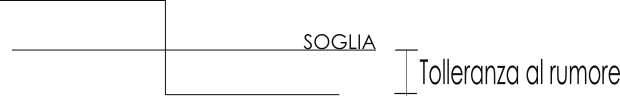
\includegraphics[width=\textwidth]{SchemaDigitale}
\chapter{Circuiti combinatori}
\section{Operatori}
\subsection{OPERATORI SEMPLICI}
Gli operatori basilari che vengono utilizzati per la costruzione di reti logiche sono i seguenti:\newline
\subsubsection*{AND}

L'operatore AND prende in input  due segnali e restituisce 1 se e solo se entrambi sono 1, altrimenti restituisce 0.
\begin{figure}[h!,right]
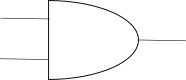
\includegraphics{AndGate}
\end{figure}
\newline Si rappresenta come : \(x*y\)\newline
\subsubsection*{OR}
\begin{figure}[h!]
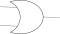
\includegraphics{OrGate}
\end{figure}
L'operatore OR prende in input due segnali e restituisce 1 se almeno uno dei due è 1, altrimenti restituisce 0.
\newline Si rappresenta come : \(x+y\)\newline
\subsubsection*{NOT}
\begin{figure}[h!]
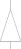
\includegraphics{NotGate}
\end{figure}
L'operatore NOT prende in input un solo segnali e restituisce 1 se il segnale è 0 e 0 se l'input è 1.
\newline Si rappresenta come : \(x'\)

\newpage
\subsection{OPERATORI COMPLESSI}
Gli operatori che vediamo di seguito possono essere considerati come operatori "complessi" ossia costituiti da elementi più semplici.
\subsubsection*{NAND}
\begin{wrapfigure}{r}{0.07\textwidth}
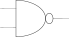
\includegraphics{NandGate}
\end{wrapfigure}
L'operatore NAND è costituito da un operatore AND seguito da un NOT.
\subsubsection*{NOR}
L'operatore NOR è costituito da un operatore OR seguito da un NOT.
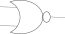
\includegraphics{NorGate}
\subsubsection*{EXOR}
L'operatore EXOR è anche detto OR esclusivo, questo perchè restituisce 1 se e solo se i due segnali in ingresso sono diversi tra loro.
\subsubsection*{EXNOR}
L'operatore EXNOR è anche detto OR inclusivo perchè restituisce 1 se e solo se i due segnali in ingresso sono uguali tra loro.
\subsubsection{RAPPRESENTAZIONE CIRCUITALE}
\newpage
\section{Algebra di boole}
Le operazioni svolte dagli operatori appena visti godono di proprietà che vanno sotto il nome di algebra di Boole. (Ognuna di esse è dimsotrabile tramite induzione completa, ossia verificando totalmente la veridicità delle implicazioni tramite tabelle di verità).
\subsection*{Proprietà distributiva}
\subsection*{Complementazione}
\subsection*{Proprietà associativa}
\subsection*{Leggi di De Morgan}
\newpage
\section{Teorema Di Shennon}
Nel processo di ricerca di un'espressione logica che impieghi gli operatori che ora conosciamo, torna utilissimo il teorema di Shennon.
Per ogni funzione logica del tipo\break\newline \( f({x_1},{x_2},{x_3},...,{x_n}) \)\break\newline vale la seguente uguaglianza.\newline \(f({x_1},{x_2},{x_3},...,{x_n})=a*f(1,{x_2},{x_3},...,{x_n})+a'*f(0,{x_2},{x_3},...,{x_n})\)\break\newline
Questa uguaglianza è valida perchè se a valesse 1, allora la parte di destra dell'OR sarà un AND con sicuramente valore 0 e quindi verrà come risultato il valore della prima espressione, altrimenti se a fosse 0 varrebbe lo stesso discorso ma al contrario.
\paragraph*{}
Procedendo iterando questo teorema sui pezzi di funzioni rimanenti si può arrivare ad un'espansione nella seguente forma:


\(f({x_1},{x_2},{x_3},...,{x_n})=a*f(1,{x_2},{x_3},...,{x_n})+a'*f(0,{x_2},{x_3},...,{x_n})\)

\newpage

\chapter{Semplificazione di funzioni logiche}
Introduciamo ora alcune definizioni:\newline\break
\textbf{Letterale}
Ogni variabile che sia affermat o negata.\break
\textbf{Minterm}
Prodotto in cui ogni variabile compare una volta come letterale.\break
\textbf{Maxterm}
Somma in cui variabile compare una volta come letterale.\break
\textbf{Implicante}
f è implicante di g se e solo se quando f è 1 allora g è 1.
\newline Si dice \textbf{implicante primo} ogni implicante che non è possibile racchiudere in uno più grande.
Essi possono essere \textbf{ridondanti} nel caso in cui coprano zone coperte da altri implicanti primi mentre altri sono invece \textbf{essenziali} perchè sono gli unici a coprire quelle zone.
\newline\break
Ogni minterm è un implicante della propria f, l'unico problema è che ognuno di essi rappresenta "pochi uni".\newline\break
Per trovare implicanti che non siano minterm è utile utilizzare la \textbf{notazione Gray}.
Essa consiste nel fare tabele di verità in cui tra ogni riga e la sua successiva c'è solamente una variabile a variare, così da poter eventualmente fare dei raccoglimenti sfruttando l'algebra di Boole.

Nel caso funzioni con più di due variabili è necessario cercare gli implicanti utilizzando altri modi per rappresentare le tabelle di verità così da far risaltare meglio le adiacenze tra i vari minterm.

Qui entra in gioco \textbf{la mappa di Karnough}

\newpage
\section{Insiemi di operatori completi ed uso delle porte logiche}

\section{Mappe a 5 e 6 variabili}
\section{Altri metodi per sintetizzare circuiti}
\section{Minimizzazione congiunta}
\newpage	
\chapter{Circuiti Combinatori Fondamentali}

Di seguito vengono rappresentati, analizzati e spiegati alcuni circuiti combinatori che sono ritenuti fondamentali in quanto compaiono molto spesso e per cui è bene ricordarsi come sono fatti per non perdere tempo.
\subsection{Multiplexer}
In generale un multiplexer è una funzione logica che tramite un criterio prende delle variabili in entrata e ne restituisce una di esse.
\subsubsection{Da 2 a 1}
Ora prendiamo in esame il più elementare tra i multiplexer, ovvero quello che fa una decisione tra due varibili in ingresso.
Questo è il più elementare perchè altrimenti avrei una variabiule in ingresso ed una in uscita e ciò non è un vera scelta.

Partiamo dalla tabella di verità scritta con il codice Grey e cerchiamone gli implicanti primi.
Partiamo da qui perchè è il punto principale per impostare come funzionerà il nostro multiplexer.

\break\nextline
\begin{tabular}{|c|c|c|c|c|}
\hline
S-AB & 00 & 01 & 11 & 10 \\ \hline
0 &    0  &  0 & 1  & 1  \\ \hline  
1 &    0  &  1 & 1  & 0  \\
\hline
\end{tabular}\break


Gli implicanti primi sono: SB, AB, S'A.
Quindi la nostra funzione può essere scritta come segue:
\( f=\) SB+S'A

Cerchiamo di capire cosa ci sta dicendo questa funzione.
Premettiamo che la convenzione che S=0 selezioni A mentre S=1 selezioni B è nostra scelta, con alcune differenze può avvenire benissimo anche il caso in cui S=0 selezioni B mentre S=1 selezioni A.

Prendendo in esame uno solo delle AND, queste ci dicono che nel caso in cui S sia 0 SICURAMENTE quel termine sarà del tutto irrilevante nel passaggio successivo costituito da un OR.
Perciò verrà selezionato ESCLUSIVAMENTE l'operazione AND che ha S=1.
Poi l'essere 0 o 1 dell'altro operando determinerà l'uscita esattamente di quel valore.

Ecco lo schema circuitale della funzione appena descritta:
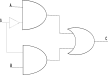
\includegraphics{Multiplexer21Circuito}
Il multiplexer 2 a 1 si rappresenta con un questo simbolo circuitale:
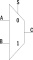
\includegraphics{Multiplexer21}
In cui i numeri indicano per quale valore di S venga selezionata la corrispondente entrata.
\subsubsection{Da 4 a 1}
Alla luce di quello che abbiamo appena letto riguardo al multiplexer 2 a 1 possiamo immaginare come realizzare questa versione più in grande.

Posso utilizzare due multiplexer 2 a 1 per ottenere due output e poi questi ultimi metterli all'interno di un ulteriore multiplexer 2 a 1 così da ottenere un solo risultato in uscita.

\(S_0_1 \) si occuperà di scremare tra A e B mentre \(S_0_2 \) scremerà tra C e D.


\subsection{Odd Function}
\subsection{Conta Uni}
\subsection{Codifica e decodifica}


\subsubsection{Decodifica per display a 7 segmenti}


\subsubsection{Priority Encoder}

\section{Indifferenze o don't care}

\chapter{Tempistiche e diagrammi temporali}

In un circuito ci sono dei ritardi tra quanto il segnale entra in una porta e quando ne esce il risultato prodotto dalla logica della porta stessa.
Questi ritardi sono dati da motivi fisici e di solito sono specificati al momento dell'acquisto della porta così da permettere di scegliere quella più adatta agli scopi per cui verrà impiegata.

I diagrammi temporali sono di due tipi:
 
\textbf{SENZA RITARDO}\newline
Quelli senza ritardi vengono impiegati per valutare la funzione logica ed effettuare operazioni di debugging se necessarie.\newline
\textbf{CON RITARDO}\newline
Quelle con ritardi invece vengono utilizzati per valutare le prestazioni della funzione logica.\newline

Un tempo utile da conoscere riguardo ad un circuito logico è quello massimo che può impiegare per restituire una risposta all'input sottopostogli.

\section{Glitch}

In un circuito possono verificarsi dei fenomeni detti \textbf{Alee o Glitch} e sono dovuti a brevi e rapidi cambiamenti di valore che avvengono con particolati combinazioni di ritardi. Influiscono sul risultato istantaneo ottenibile dal circuito (transitorio) ma non sulla correttezza della funzione logica.


Per ovviare a ciò si utilizza la tipologia di\textbf{ circuito sincrono}

\subsection{Alee su Karnaugh}

\chapter{Circuiti aritmetici}

Si chiamano \textbf{circuiti aritmetici} tutti quei circuiti che sfruttano porte logiche e il sistema di numerazione binario per effettuare operazioni di calcolo.


\section{Struttura iterativa generica}

\section{Somma}

\subsection*{Half adder}
Iniziamo con la tabella di verità del circuito che dovrebbe sommare due ingressi da 1 bit ciascuno.
Esso restituirà un risultato con 2 bit in uscita.
Indichiamo con a e b i due ingressi, mentre con s il bit meno significativo del risultato e con c quello più significativo.
La lettera c ci ricorderà anche tale cifra è dovuta al carry dell'operazione.
\newline
\begin{tabular}{|c|c|c|c|}
\hline
a & b & c & s \\ \hline
0 & 0 & 0 & 0 \\ \hline
0 & 1 & 0 & 1 \\ \hline
1 & 1 & 1 & 0 \\ \hline
1 & 0 & 0 & 1 \\ 
\hline
\end{tabular}



Mettendo s e c in due mappe di Karnaugh separate si possono costruire le funzioni logiche di ognuno.
Iniziamo con S:

\begin{tabular}{|c|c|c|}
\hline
a/b & 0 & 1 \\ \hline
0   & 0 & 1 \\ \hline
1   & 1 & 0 \\ \hline
\end{tabular}

La funzione logica che rappresenta l'uscita s quindi è aXORb

Passando a C otteniamo poi:

\begin{tabular}{|c|c|c|}
\hline
a/b & 0 & 1 \\ \hline
0   & 0 & 0 \\ \hline
1   & 0 & 1 \\ \hline
\end{tabular}

La funzione logica che esprime il comportamento di C è aANDb

Il circuito dell'half adder è:


\subsection*{Full adder}




\subsection*{Prestazioni}

\section{Sottrazione}
\section{Moltiplicazione}




\chapter{Linguaggi di descrizione dell'hardware}
\section*{VHDL}

Il linguaggio che utilizzeremo è il \textbf{VHDL}, ossia \textbf{V}ery highspeed integrated circuit \textbf{H}ardware \textbf{D}escription \textbf{L}anguage.

Il VHDL ci permette di lavorare secondo 3 \textbf{metodologie}

\begin{itemize}
\item \textbf{Top-Down}
\item \textbf{Buttom-Up}
\item \textbf{Meet In The Middle}
\end{itemize}

e secondo 3 viste

\begin{itemize}
\item \textbf{Data flow}: \newline Consiste nella descrizione delle uscite in funzione degli ingressi. E' specificata con equazioni booleane messe a sistema tra loro.
\item \textbf{Strutturale}:\newline Consiste nella descrizione del circuito grazie all'utilizzo di componenti già esistenti che verranno combinati ed aggregati tra di loro. 
\item \textbf{Comportamentale}: \newline Consiste nella descrizione del circuito tramite l'algoritmo che dovrà implementare.
\end{itemize}


\newpage
\subsection*{Entità}

La nozione di \textbf{entità} in VHDL corrisponde alla rappresentazione di un blocco \textbf{SENZA SPECIFICARNE} la logica interna.

Esso specifica :

\begin{itemize}
\item \textbf{nome}
\item \textbf{numero di ingressi}
\item \textbf{numero di uscite}

\end{itemize}

Di seguito il codice per dichiarare un'entità di nome nome_entity con n ingressi e m-n uscite.

\begin{verbatim}

entity nome_entity is
port
(	
	nome_porta1 : tipo_ingresso,
	nome porta2 : tipo_ingresso,...
	nome_portan : tipo_ingresso;
	nome_portan+1 : tipo_uscita,
	nome_portan+2 : tipo_uscita,...
	nome_portan+3 : tipo_uscita;
);
end  nome_entity;

\end{verbatim}


\subsection*{Architettura}

La nozione di \textbf{architettura} in VHDL specifica il comportamento di un'entità.
(Ad un'entità possono corrispondere più architetture.)


\subsection*{Testbench}

Il \textbf{testbench} è un'unione della vista dataflow con quella strutturale che permette la simulazione del circuito dando dei dati in ingresso.

\subsection*{Operatori,Identificatori e operazioni multiple}

VHDL possiede tutte le operazioni booleane come and,or,xor...\break\nextline
La precedenza maggiore tra tali operazioni la ha la porta NOT mentre a differenza di quello che avviene nell'algebra booleana il resto degli operatori ha la stessa priorità perciò per forzare alcune operazioni prima di altre bisogna usare le parentesi !\nextline
Nella descrizione delle architetture a volte è necessario instanziare variabili interne, queste vengono chiamate \textbf{signal} e necessitano di un nome univoco per essere riconosciuti nello svolgimento della logica del componente.\break\nextline
(Attenzione che VDHL NON è case sensitive).

All'interno della stessa architettura possono avvenire più operazioni. L'ordine in cui vengono specificate all'interno dell'architettura non è rilevante perchè vanno concepite come un sistema in cui procedono in parallelo.










































































































\end{document}